Databázových systému (systémů řízení báze dat, zkráceně SŘBD) existuje nepřeberné množství.
\footnote{\label{rdbms_list}\url{http://en.wikipedia.org/wiki/List_of_relational_database_management_systems}}
\footnote{\url{http://en.wikipedia.org/wiki/List_of_object_database_management_systems}}
Jednotlivé SŘBD můžeme můžeme dělit dle různých kritérií. Nejčastějším kritériem, dle kterého jsou SŘBD děleny, je jejich datový model.
Ten popisuje základní strukturu dat, to jak jsou data uložena, uspořádána, jejich sémantiku, vztahy mezi daty a jejich integritní omezení. Datový model umožňuje popsat návrh databáze na její fyzické i logické úrovni.\cite[s.~945--964]{korth:dbsc}

Typů databází dle jejich datového modelu existuje celá řada. Já se zde omezím jen na základní čtyři, které jsou uplatněny v této práci.

\section{Entity-relationship model}
\emph{Entity-relationship} (\textbf{E-R}) datový model využívá kolekce jednoduchých objektů, nazývaných entity, a vztahů mezi těmito entitami. Entita je abstrakcí nějaké věci nebo objektu z reálného světa, která je jednoznačně odlišitelná od ostatních objektů. 

Entity-relationship datový model je široce využíván při databázovém návrhu. Výsledkem návrhu jsou diagramy, které se nazývají \emph{entity-relationship diagramy} (\textbf{ERD}).
\begin{figure}[h]
  \begin{center}
    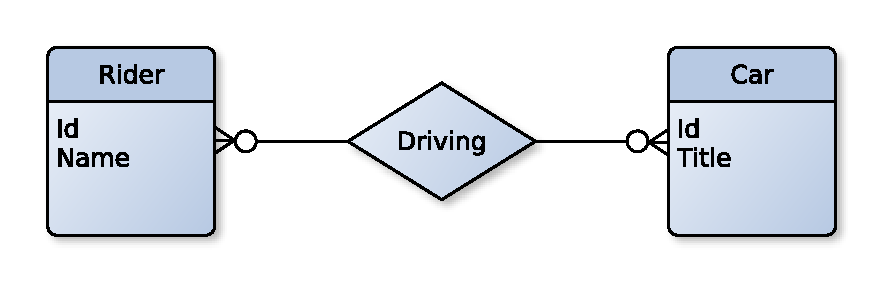
\includegraphics[width=40em]{obr/era}
    \caption{Ukázka ER diagramu}
    \label{fig:era}
  \end{center}
\end{figure}
\section{Relační databáze}
Relační databáze jsou založeny na relačním modelu a jsou v součastnosti nejvíce používanými \footnote{\label{dbms_rank}\url{http://db-engines.com/en/ranking}} SŘBD. Díky svému snadnému použití a pochopení, nahradily relační databáze své předchůdce. Předchůdci relačních databází byly datbáze síťové a hierarchické.
\subsection{Datový model}
Relační databáze využívají relační datový model. Ten je nejrozšířenějším používaným datovým modelem dnešení doby a velká část součastných databázových systému je založena právě na tomto datovém modelu.

Relační model je založen na kolekcích tabulek, kterých se využíva jak pro reprezentaci dat (tabulky \texttt{RIDER} a \texttt{CAR} na obrázku \ref{fig:rel_model}), tak i pro vztahy mezi těmito daty (tabulka \texttt{CAR\_RIDER} na obrázku \ref{fig:rel_model}). Každá tabulka má několik sloupců, kde každý sloupec (též označován jako atribut) má svůj unikátní název (identifikátor), typ a rozsah neboli doménu.
\begin{figure}[h]
  \begin{center}
    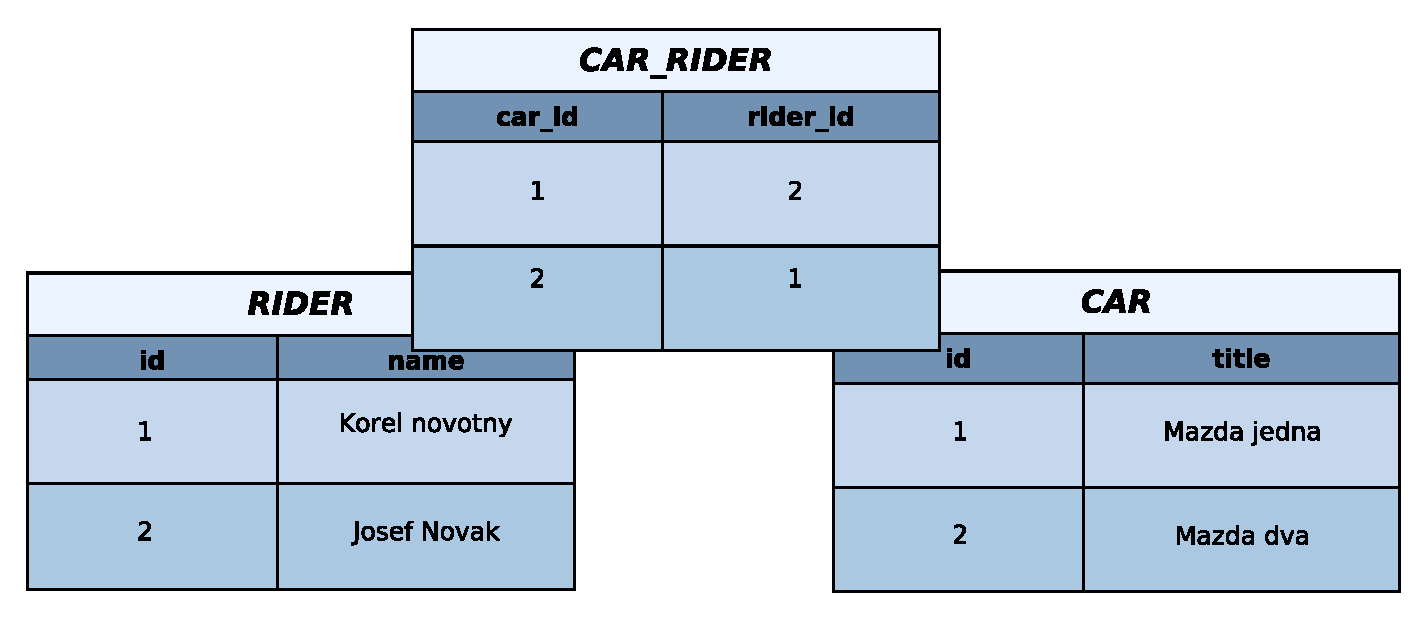
\includegraphics[width=40em]{obr/rel_model}
    \caption{Relační datový model}
    \label{fig:rel_model}
  \end{center}
\end{figure}
\subsection{Dotazovací jazyk}
Standardem pro práci s relačními datbázemi se stal jazyk \emph{\textbf{S}tructured \textbf{Q}uery \textbf{L}anguage} (\textbf{SQL}). Ačkoliv všechny hlavní relační databáze používají standardizovaný jazyk SQL, tak mezi nimi není zcela zaručena přenositelnost jednotlivých dotazů. Důvodem jsou hlavně různá rozšíření a vylepšení, kterými se od sebe různé produkty odlišují a také to, že ne všechny produkty implementují kompletní normu jazyka SQL.

Poslední normou jazyka SQL, která se týká čistě relačních dat a operací, je norma SQL-92 (někdy se uvádí i název SQL2), tato norma aktualizovala původní normu známou pod názvem SQL-86.
\subsection{Zástupci}
Systémů řízení báze dat, stavějících na relačním datovém modelu, je celá řada\cref{rdbms_list}. Následující seznam zástupců je rozdělen na dvě kategorie. Na zástupce ze světa OSS a na komerční produkty. Jednotliví zástupci jsou řazeni sestupně dle jejich popularity \cref{dbms_rank}.
\begin{enumerate}
  \item OSS řešení
  \begin{itemize}
    \item MySQL
    \item PostgreSQL
    \item SQLite
    \item Firebird
  \end{itemize}
  \item Komerční řešení
  \begin{itemize}
    \item Oracle
    \item Microsoft SQL Server
    \item Microsoft Access
    \item Db2
  \end{itemize}
\end{enumerate}
\section{Objektově-relační databáze}
S rozmachem programovacích jazyků podporujících objektově orientované programování (\emph{OOP}, bylo třeba řešit problém persistence objektů a netriviálních datových struktur. Objektově-relační databáze byly jednou z odpovědí na tento problém (další řešení je použití objektové datbáze nebo objektově relační mapování). Objektově-relační databáze jsou jen rozšířenou variantou oproti relačním databázím, tudíž většina zmíněných relačních datbází podporuje do jisté míry i objektově-relační přístup.
\subsection{Datový model}
Jedná se o relační model, který je rozšířený o vlastní (abstraktní) datové typy s podporu dědičnosti a metod. Dotazovací jazyk je zde upraven (rozšířen) tak, že podporuje dotazy nad těmito typy.\cite[s.~945--964]{korth:dbsc}

\section{Objektové databáze}
Objektové databáze, jak již bylo naznačeno, jsou další odpovědí na řešení problému, ukládání, vyhledávání a manipulování s daty v OOP jazycích. Oproti objektově-relačním databázím se jedná o zcela jíný přístup se zcela jiným datovým modelem, bez jakékoliv návaznosti na relační model.

\subsection{Datový model}
Na objektově orientovaný datový model můžeme nahlížet, jako na E-R datový model, rozšířený o některé prvky OOP. Těmito prvky jsou: zapouzdření, metody (funkce), dedičnost, polymorfismus a identita objektu.

\subsection{Dotazovací jazyk}
Narozdíl od relačních a objektově-relačních databází, zde neexistuje jednotný normalizovaný jazyk, pro práci s uloženými daty. Což hodnotím jako jedno z největších úskalí u tohoto typu databází. A zřejmě je to i jeden z hlavních důvodů proč se objektové databáze teší menší popularitě než relační databázové systémy podporující SQL.
 
\subsection{Zástupci}
Oproti relačním databázím, existuje podstatně méně produktů využívajících objektový datový model. Následuje přehled některých z nich.
\begin{enumerate}
  \item OSS řešení
  \begin{itemize}
    \item Db4o
    \item NeoDatis
    \item ZODB
  \end{itemize}
  \item Komerční řešení
  \begin{itemize}
    \item Caché
    \item Objectivity/DB
    \item ObjectDB
    \item Versant Object Database
    \item JADE
  \end{itemize}
\end{enumerate}

\section{NoSQL databáze}
NoSQL databáze není jeden určitý druh databáze, ale označuje se tak celá skupina databází, která nestaví na relačním modelu dat, a kde jednotlivé databáze negarantují všechny ACID vlastnosti. Mezi NoSQL databáze by se daly zařadit i objektově orientované databáze.

Zkratka NoSQL se někdy pojí s pojmem "`Not Only SQL"', čímž se dává najevo, že některé z NoSQL databází podporují i SQL dotazy.

\subsection{Datový model}
Jelikož je NoSQL pojmem zastřešujícím celou řadou ruzných datábází s určitými společnými vlastnostmi, neexistuje zde pouze jen jeden datový model, ale existuje jich hned několik. Ale pro zjednodušení se dají všechny tyto datové modely označit jako semi-structured datový model.
\subsubsection{Semi-structured}
Jedná se o specialní datový model, odlišující se od ostatních datových modelů tím, že umožnuje ukládat záznamy stejného typu s odlišnou množinou atributů.

Nejznámějšími formáty reprezentující tento model jsou e\textbf{X}tensible \textbf{M}arkup \textbf{L}anguage (\emph{XML}) a \textbf{J}ava\textbf{S}cript \textbf{O}bject \textbf{N}otation (\emph{JSON}).

\subsection{Dotazovací jazyk}
Platí zde to samé co u objektových databází, tedy že zde neexistuje jednotný normalizovaný jazyk - způsob jak k datům přistupovat, či je modifikovat. Vyjímkou jsou některé NoSQL databáze, které podporují i SQL jazyk. A je tedy možno s danou datbází a jejími daty pracovat pomocí SQL dotazů.

\subsection{Zástupci}
NoSQL databází existuje velké množství. Mezi nejznámější patří tyto:
\begin{itemize}
  \item MongoDB -- dokumentová databáze (BSON)
  \item Cassandra -- wide column store 
  \item Redis -- asociativní pole
  \item HBase -- wide column store 
  \item CouchDB -- dokumentová databáze (JSON)
  \item Neo4j -- grafová databáze
\end{itemize}
